\section{Modeling and systematic uncertainties}
\lb{sec:lowE_syst}

In this appendix we study the dependence of the spectrum of gamma-ray emission at the base of the FB
on the selection of the low energy range in the definition of the diffuse foreground model
and on the choice of the class of the events (UltraCleanVeto vs Source).
We use the rectangles model of the FB in Section \ref{sec:box_model}
as our baseline example.
In this model, the foreground emission template consists of Source data averaged over the energy interval $0.3 - \SI{1.0}{GeV}$. 
To probe the dependence on the choice of the low-energy range in the model, 
we pick three non-overlapping energy ranges $0.3 - \SI{0.5}{GeV}$, $0.5 - \SI{1.0}{GeV}$, and $1.0 - \SI{2.2}{GeV}$ 
and use the same analysis as for the baseline model. 
We also compare with the spectra obtained using UltraCleanVeto data both in the definition of the model
at low energies and in the analysis at high energies.
The residual spectra resulting from the different energy ranges and data classes are shown in Figure \ref{fig:syst_models}. 
The agreement among the models is relatively good at $E > 10$ GeV, especially for negative longitudes.

As one can see from Figure \ref{fig:syst_models}, the last data point in the negative longitudes may have an upwards statistical fluctuation,
which can influence the conclusions about the lower limit in the cutoff values.
In order to test this dependence, we exclude the last energy bin $680\;{\rm GeV} - 1\;{\rm TeV}$ and 
repeat the derivation of the best-fit parameters in the rectangles model of the FBs.
The results are presented in Table \ref{tab:param2}.
Without the last data point, the four areas with ``infinite'' cutoff energy have now a finite cutoff,
but with a significance $-2\Delta \log L  < 1$, i.e., the models are still consistent with a simple power law.
The 95\% confidence lower limit on the cutoff value is also smaller for the data set without the last point,
but in this case we are using the data up to 680 GeV rather than 1 TeV.

\begin{figure*}[h]
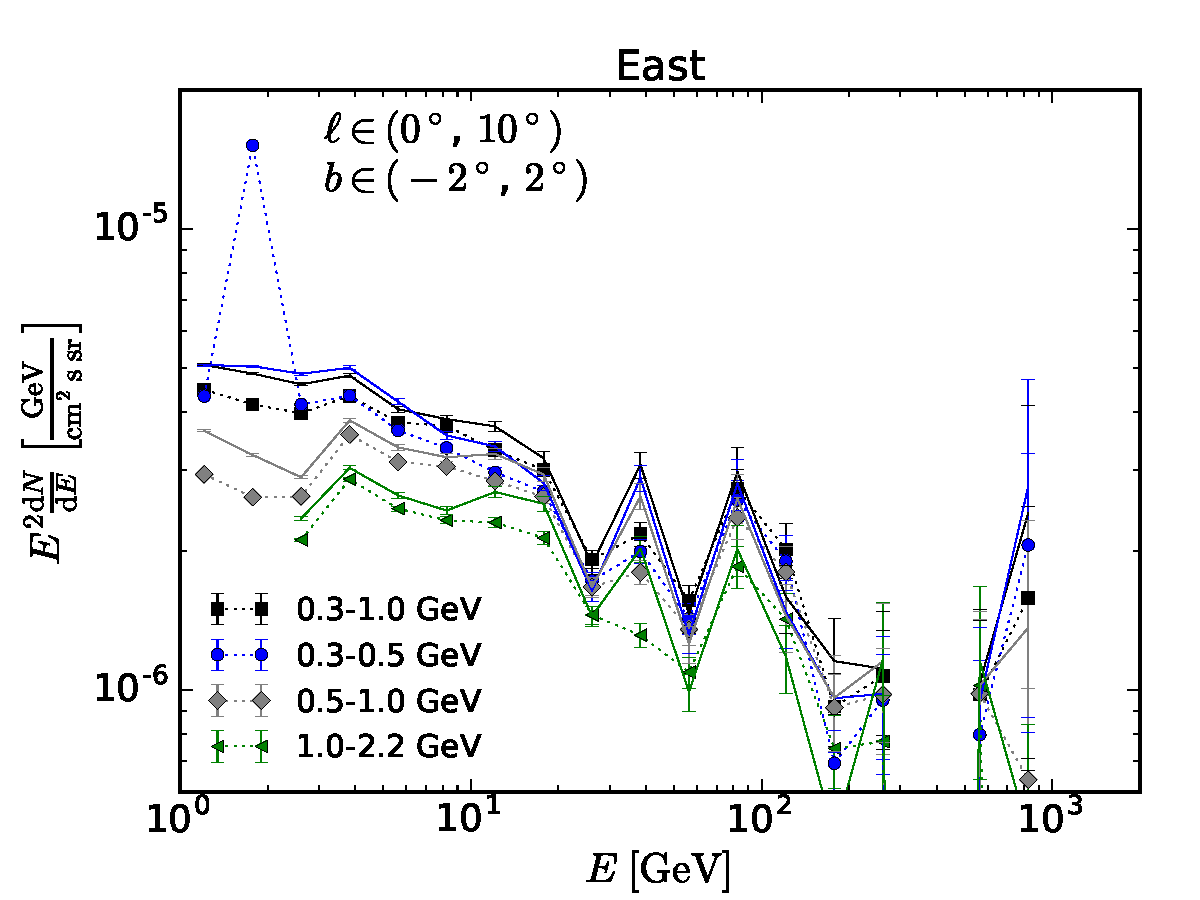
\includegraphics[width=0.5\textwidth]{plots/SED_different_lowE_ranges_boxes_l=5_b=0.pdf}
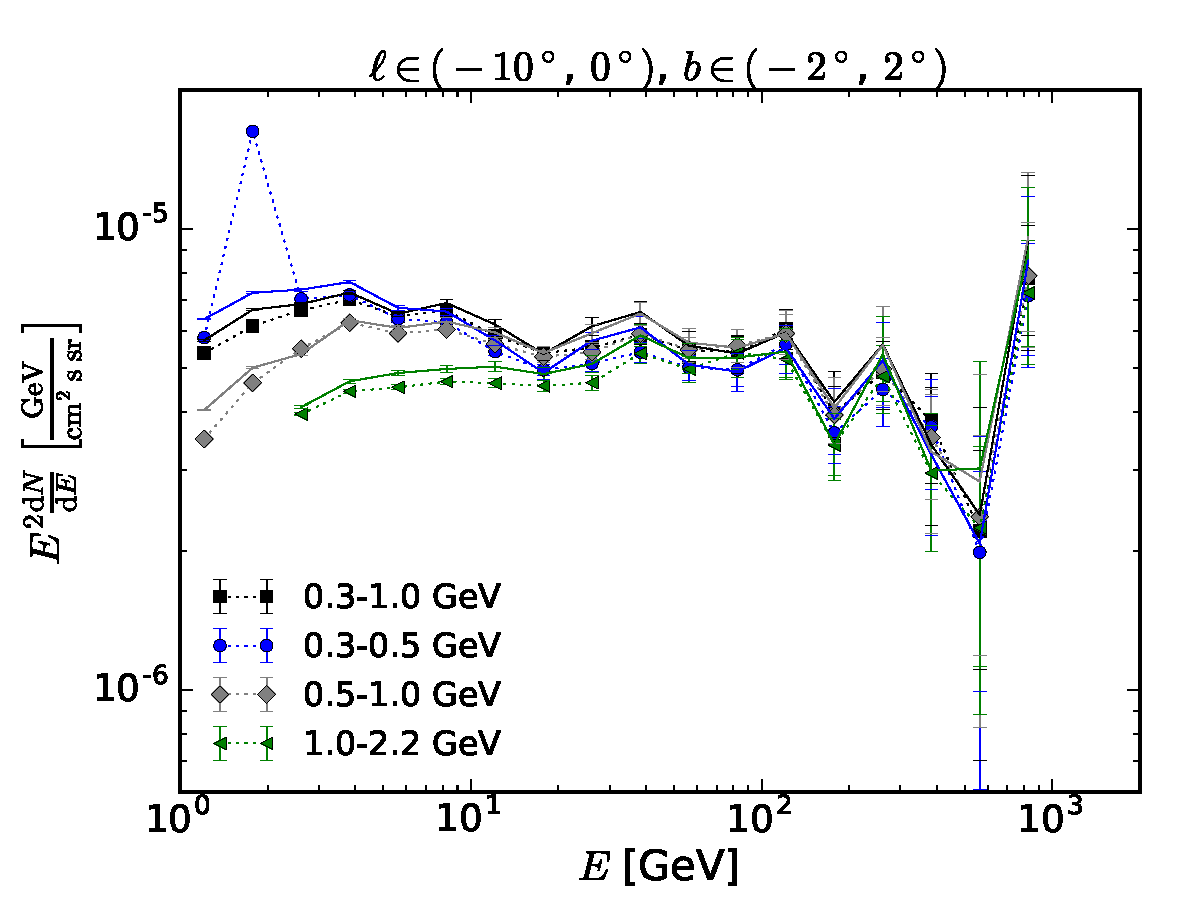
\includegraphics[width=0.5\textwidth]{plots/SED_different_lowE_ranges_boxes_l=-5_b=0.pdf}
\caption{SED of the residual in the rectangles model using Source class (dotted lines with markers) and UltraCleanVeto class data (solid lines) 
in four different energy ranges used to determine the foreground diffuse emission template. 
The baseline model, presented in Section \ref{sec:box_model}, has the low-energy range in the definition of the foreground model
$0.3 - \SI{1.0}{GeV}$ (black squres).}
\label{fig:syst_models}
\end{figure*}

\begin{comment}
\section{Fraction of masked pixels}

\begin{figure*}[h]
\centering
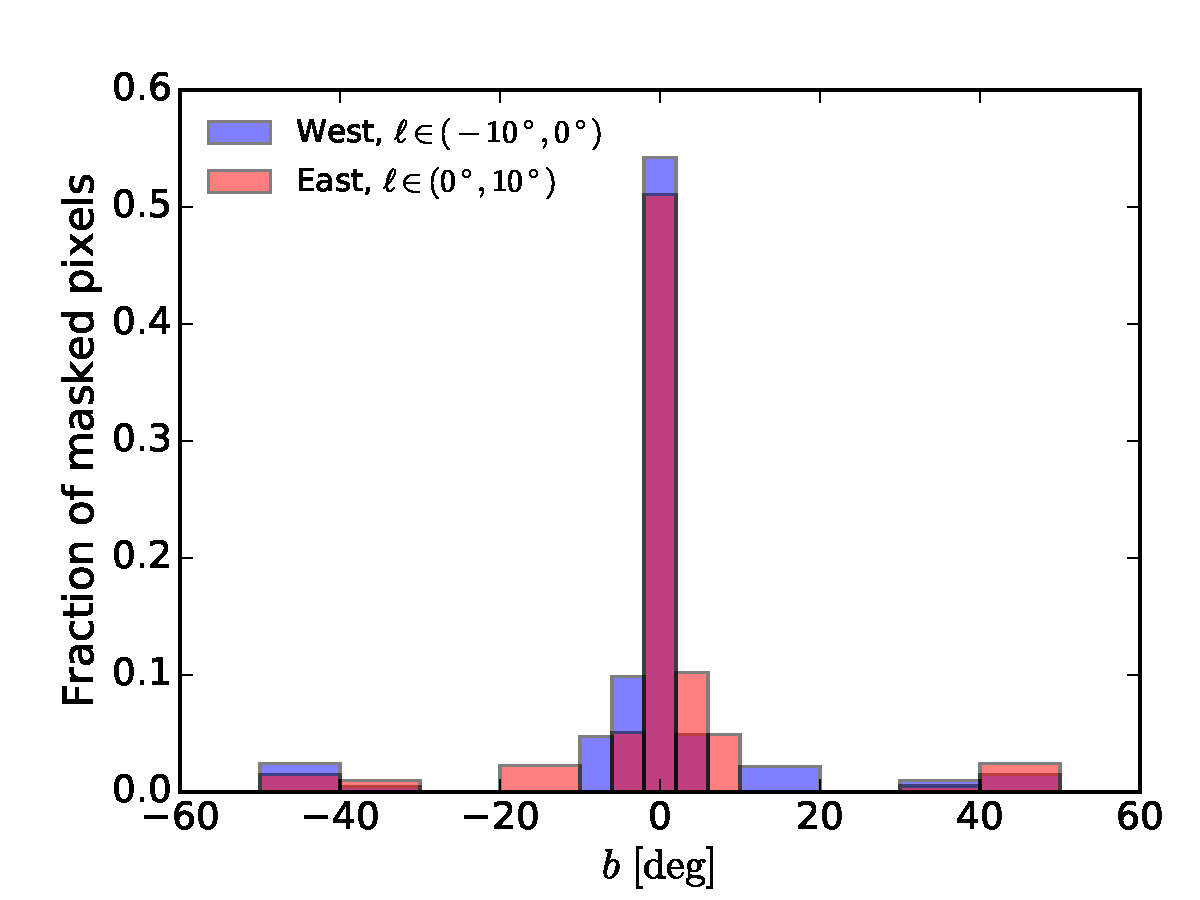
\includegraphics[width=0.5\textwidth]{plots/Fraction_masked_pixels.pdf}
\caption{Masked pixels.}
\label{fig:masked_pixels}
\end{figure*}
\end{comment}



\begin{table*}
  \begin{center}
    \caption{Best-fit parameters of the rectangles model without the last energy bin: $680\;{\rm GeV} - 1\;{\rm TeV}$.
    The definitions of the columns are the same as in Table \ref{tab:param}.
    \lb{tab:param2}
    }
        \begin{tabular}{|c|c|c|c|c|c|c|c|} % <-- Alignments: 1st column left, 2nd middle and 3rd right, with vertical lines in between
     	\hline
		 Lat & Lon  & $N_0$ & $n$ & $E_{\rm cut}$ &  $-2 \Delta \log \La$ & $E_{\rm cut, 95\%}$ & $E_{\rm cut, 95\%}^{\rm min}$ \\ 
		     &        &  {\small $\SI{e-6}{GeV^{-1}cm^{-2}s^{-1} sr^{-1}}$ }&  & {\small $\SI{}{GeV}$ }& &{\small  $\SI{}{GeV}$ }&{\small  $\SI{}{GeV}$ }\\ 
		\hline
  		$(\ang{2}, \ang{6})$ & $(\ang{0}, \ang{10})$ & 1.9 & 1.9 & 45 & 6.8 &25 & 25\\ 
		& $(\ang{-10}, \ang{0})$ & 2.0 & 2.2 & 690 & 0.45 & 210 & 210\\ 
 		\hline
  		$(\ang{-2}, \ang{2})$ & $(\ang{0}, \ang{10})$ & 3.6 & 2.3  & 610 & 0.42 & 180 & 2.0 \\ 
		& $(\ang{-10}, \ang{0})$ & 6.4 & 2.1 & 1.3e3 & 0.76 & 480 & 460\\ 
 		\hline
  		$(\ang{-6}, \ang{-2})$ & $(\ang{0}, \ang{10})$ & 1.8 & 2.1 & 260 & 3.4 & 130 & 2.3  \\ 
		& $(\ang{-10}, \ang{0})$ & 2.9 & 2.1 & 780 & 0.96 & 290 & 290\\ 
 \hline
    \end{tabular}
  \end{center}
\end{table*}
